\documentclass[../main.tex]{subfiles}
\usepackage[utf8]{inputenc}
\usepackage[T1]{fontenc}
\usepackage{graphicx}
\usepackage{longtable}
\usepackage{wrapfig}
\usepackage{rotating}
\usepackage[normalem]{ulem}
\usepackage{amsmath}
\usepackage{amssymb}
\usepackage{capt-of}
\usepackage{hyperref}
\usepackage{float}
\graphicspath{{../}}
\author{Cezary Wieczorkowski}
\date{\today}
\title{Brevitas}
\hypersetup{
 pdfauthor={Cezary Wieczorkowski},
 pdftitle={Brevitas},
 pdfkeywords={},
 pdfsubject={},
 pdflang={Polish}}
\begin{document}


\section{Brevitas}

\subsection{Wprowadzenie do sieci CNN}

Splotowe sieci neuronowe są typem sieci neuronowych szeroko stosowanym przy rozpoznawaniu oraz śledzeniu obiektów. Szczególną właściwością tej
klasy sieci neuronowych jest fakt, że wykrywają one użyteczne aspekty danych wejściowych poprzez hierarchiczną strukturę kerneli (filtrów). W ten sposób pierwsze warstwy sieci
wykrywają bardziej ogólne wzory natomiast głębsze warstwy skupione są na wykryciu coraz to bardziej konkretnych wzorów \cite{presentation_cnn}.

\subsubsection{Struktura sieci splotowych}

Splotowe sieci neuronowe składają się z szeregu połączonych warstw o różnych funkcjach. Kolejność oraz ilość połączonych warstw zależy od implementacji konkretnej sieci.
W celu klasyfikacji obrazu, wartości pikseli obrazu podawane są jako macierz wejściowa sieci neuronowej gdzie propagując przez kolejne warstwy sieci aż do jej wyjścia którym może być prosta klasyfikacja obrazu do konkretnej
kategorii lub dodatkowo lokalizacja wykrywanego obiektu w obrębie klasyfikowanego obrazu.

\begin{itemize}
    \item Warstwa splotowa
    \item Wastwa pooling
    \item Warstwa aktywacyjne
    \item Warstwy normalizacyjne
    \item Warstwa w pełni połączona
\end{itemize}

\subsubsection{Warstwy konwolucyjne}

Warstwa splotowa jest kluczowa w działaniu sieci, tutaj zachodzi detekcja wyuczonych obiektów w obrazie. Warstwa ta wykonuje operacje splotu \ref{fig:conv_layer} pikseli obrazu wejściowego z filtrami których wartości (wagi) są determinowane w procesie 
uczenia sieci.

\begin{figure}[H]
    \centering
    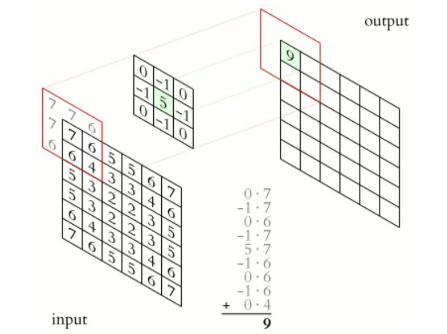
\includegraphics[scale=0.6]{conv.png}
    \caption{Ilustracja działania warstwy splotowej}
    \label{fig:conv_layer}
\end{figure}

Rozmiar danych wyjściowych z tej warstwy będzie pomniejszony o wysokość oraz szerokość filtru odjąć jeden.

\subsubsection{Warstwy pooling}

W przypadku konieczności redukcji rozmiaru macierzy przechodzącej przez sieć stosuje się warstwy pooling. Warstwa ta podobnie jak warstwa splotowa działa na zasadzie filtru poruszającego się po danych wejściowych
jednak w tym przypadku filtr nie posiada wag służy jedynie do wyróżnienia danego obszaru macierzy wejściowej. Dana wyjściowa dla obszaru objętego filtrem jest determinowana przez typ poolingu. Najczęściej stosowane są
Max pooling - gdzie na wyjściu znajdzie się najwyższa wartość objęta filtrem oraz Avarage pooling gdzie wyjście będzie średnią arytmetyczną wartości objętych filtrem.

\begin{figure}[H]
    \centering
    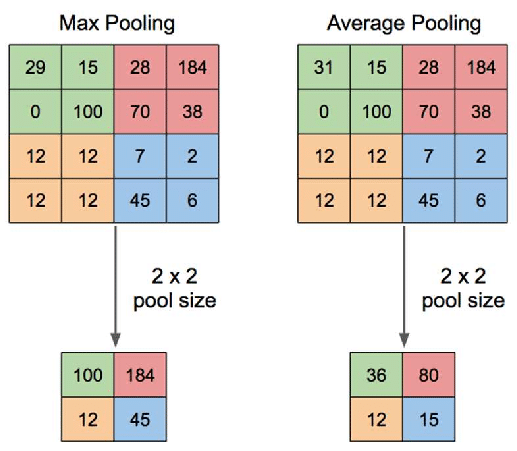
\includegraphics[scale=0.6]{pooling.png}
    \caption{Ilustracja działania warstwy pooling dla filtru 2x2}
    \label{fig:pooling}
\end{figure}

\subsubsection{Warstwy aktywacyjne}

Warstwy aktywacyjne najczęściej występują zaraz po warstwach splotowych. Mają one na celu poprawę procesu uczenia poprzez wprowadzenie do sieci efektu nieliniowości. Często używaną funkcją aktywacyjną jest ReLU mająca postać:

\begin{equation}
    ReLU(x) = max(0,x)
\end{equation}

\subsubsection{Warstwy normalizacyjne}

Warstwy normalizacyjne mają za zadanie utrzymać wartości będące wyjściem poprzedzających je warstw w zadanym zakresie. Osiągane jest to poprzez normalizację oraz skalowanie wartości wejściowych warstwy. Dzięki
temu poprawiana jest stabilność uczenia \cite{Setto2021FPGA_CNN}. Dodatkowo w przypadku złożonych sieci neuronowych warstwy normalizacyjne zapobiegają przekroczeniu wartości maksymalnej lub minimalnej dla wyjść kolejnych neuronów w sieci.

\subsubsection{Warstwy w pełni połączone}

Jest to najczęściej ostatnia warstwa sieci neuronowej, zamienia ona macierz będącą wyjściem poprzednich warstw na końcowy wektor wyjściowy sieci. Liczba elementów wektora zależy od ilości klas obiektów w danej sieci.

\subsection{Trening sieci przy pomocy Brevitas}

W celu zwiększenia efektywności obliczeniowej a także zmniejszenia jej zapotrzebowania na pamięć należy przeprowadzić proces kwantyzacji. Proces ten polega na zamianie liczb reprezentujących wagi w sieci neuronowej
z zmiennoprzecinkowych na liczby całkowite o stałej liczbie bitów. Powoduje to spadek dokładności sieci ale skutkuje też znacznym uproszczeniem procesu obliczeniowego oraz zapotrzebowania sieci na pamięć. Kwantyzacje sieci można
przeprowadzić już na etapie treningu co nazywamy Quantization aware training. Biblioteka Brevitas \cite{brevitas} została opracowana przez firmę Xilinx z myślą o kwantyzacji sieci neuronowych w celu implementacji na układach FPGA.
Biblioteka ta jest oparta na popularnym frameworku uczenia maszynowego PyTorch \cite{NEURIPS2019_9015}. Posiadając kod sieci używającej PyTorch proces kwantyzacji podczas treningu polega na podmianie instancji klasycznych
warstw z biblioteki PyTorch na ich skwantyzowane implementacje z biblioteki Brevitas.


\end{document}